\ifx\wholebook\relax \else
% ------------------------

\documentclass[b5paper]{ctexart}
\usepackage[nomarginpar
  %, margin=.5in
]{geometry}

\addtolength{\oddsidemargin}{-0.05in}
\addtolength{\evensidemargin}{-0.05in}
\addtolength{\textwidth}{0.1in}

\usepackage[cn]{../../../prelude}

\setcounter{page}{1}

\begin{document}

\title{基数树}

\author{刘新宇
\thanks{{\bfseries 刘新宇 } \newline
  Email: liuxinyu95@gmail.com \newline}
  }

\maketitle
\fi

\markboth{基数树}{基本算法}

\ifx\wholebook\relax
\chapter{基数树}
\numberwithin{Exercise}{chapter}
\fi

%\section{简介}
\label{introduction} \index{基数树}

排序二叉树将信息存储在节点中。我们可以用边(edge)来携带信息么?基数树(Radix tree),包括trie、前缀树、后缀树就是根据这一思路设计出的数据结构。它们产生于1960年代,被广泛用于编译器\cite{okasaki-int-map}和生物信息处理(如DNA模式匹配)\cite{wiki-suffix-tree}等领域。

\begin{figure}[htbp]
  \centering
  \includegraphics[scale=0.4]{img/radix-tree.ps}
  \caption{基数树}
  \label{fig:radix-tree}
\end{figure}

图\ref{fig:radix-tree}展示了一棵基数树。它包含了二进制串1011、10、011、100、0。如果查找二进制数$k=(b_0b_1...b_n)_2$,我们首先检查左侧的最高位$b_0$。若为0,则转向左子树继续查找;若为1,则转向右子树。接着,我们检查第二位,并重复这一过程直到处理完所有的$n$位或到达某一叶子节点。我们并不需要在节点中存储键(key),这一信息由边来代表。图\ref{fig:radix-tree}标注在节点中的键仅仅是为了示意。对于整数类型的键,我们可以使用二进制,并利用位运算进行操作。

\section{整数trie}
\label{int-trie} \index{基数树!整数trie}

我们称图\ref{fig:radix-tree}所示的数据结构为\emph{binary trie}。Trie是Edward Fredkin在1960年提出的。它来自英文单词re\textbf{trie}val。Fredkin将其读作/'tri:/,但其他人读作/'trai/(和英文单词try的发音相同)\cite{wiki-trie}。有些情况下trie也被称为前缀树,在本章中,trie和前缀树分指不同的数据结构。一棵binary trie是一种特殊的二叉树,每个键的位置由它的二进制位来决定。0表示“向左”,1表示“向右”\cite{okasaki-int-map}。考虑图\ref{fig:big-endian-trie}中的trie,3个不同串``11''、``011''、``0011''代表同一个十进制整数3。

\begin{figure}[htbp]
  \centering
  \includegraphics[scale=0.4]{img/big-endian-trie.ps}
  \caption{大端(big-endian)trie}
  \label{fig:big-endian-trie}
\end{figure}

如果把前面的0也当作有效位,在一个32位整数的系统中,向空trie插入1,结果将是一棵32层的树。为了解决这一问题,Okasaki建议使用小端整数\cite{okasaki-int-map}。二进制数的最高位(MSB)通常在左边,最低位(LSB)在右边。这种形式称为大端整数,反之最高位在右边称为小端整数。使用小端,1表示为$(1)_2$,、2表示为$(01)_2$、3表示为$(11)_2$……

\subsection{定义}
我们可以重用二叉树的定义。一个节点要么为空,要么包含左右子树和一个值(值可以为空)左子树编码为0,右子树编码为1。

\lstset{frame = single}
\begin{Haskell}
data IntTrie a = Empty
               | Branch (IntTrie a) (Maybe a) (IntTrie a)
\end{Haskell}

对于binary trie中的任一节点,其对应的整数键是由节点的位置唯一确定的。因此我们无需在节点中存储键,而只需存储值。键的类型被固定为整数,如果值的类型为$A$,则树的类型为$IntTrie\ A$。

\subsection{插入}
\index{整数trie!插入}

当插入整数键$k$和值$v$时,我们将$k$转换成二进制。如果$k$是偶数,最低位是0,我们递归向左子树插入;如果$k$是奇数,最低位是1,我们递归向右子树插入。接下来我们将$k$除以2取整以去掉最低位。对于非空的trie树$T = (l, v', r)$,其中$l$、$r$是左右子树,$v'$是值(可为空),函数$insert$的定义如下:

\be
\begin{array}{rcl}
insert\ \nil\ k\ v & = & insert (\nil, \textit{Nothing}, \nil)\ k\ v \\
insert\ (l, v', r)\ 0\ v & = & (l, \textit{Just}\ v, r) \\
insert\ (l, v', r)\ k\ v & = & \begin{cases}
  even(k): & (insert\ l\ \dfrac{k}{2}\ v, v', r) \\
  odd(k) : & (l, v', insert\ r\ \lfloor \dfrac{k}{2} \rfloor\ v) \\
\end{cases}
\end{array}
\ee

如果$k = 0$,我们将$v$存入节点。如果$T = \nil$,结果为$(\nil, \textit{Just}\ v, \nil)$。只要$k \neq 0$,我们就根据$k$的奇偶性前进,遇到$\nil$就建立一个空叶子节点$(\nil, \textit{Nothing}, \nil)$。如果$k$已经存在,这一算法覆盖以前的值。我们也可以用一个列表存储多个值,并将$v$添加到列表中。图\ref{int-trie}的例子是依次插入映射\{$ 1 \rightarrow a, 4 \rightarrow b, 5 \rightarrow c, 9 \rightarrow d$\}的结果。下面的例子程序实现了$insert$函数:

\begin{figure}[htbp]
  \centering
  \includegraphics[scale=0.5]{img/int-trie.ps}
  \caption{小端整数trie,包含映射:
          \{$ 1 \rightarrow a, 4 \rightarrow b, 5 \rightarrow c, 9 \rightarrow d$\}}
  \label{fig:int-trie}
\end{figure}

\begin{Haskell}
insert Empty k x = insert (Branch Empty Nothing Empty) k x
insert (Branch l v r) 0 x = Branch l (Just x) r
insert (Branch l v r) k x | even k    = Branch (insert l (k `div` 2) x) v r
                          | otherwise = Branch l v (insert r (k `div` 2) x)
\end{Haskell}

为了判定一个数的奇偶性,我们可以判断它除以2的余数(模2)是否为0:$even(k) = (k \bmod 2 = 0)$,或者使用位运算,如:\texttt{(k \& 0x1) == 0}。我们也可以消除递归用循环实现插入算法:

%\begin{algorithm}
\begin{algorithmic}[1]
\Function{Insert}{$T, k, v$}
  \If{$T =$ NIL}
    \State $T \gets$ \Call{Empty-Node}{}  \Comment{(NIL, Nothing, NIL)}
  \EndIf
  \State $p \gets T$
  \While{$k \neq 0$}
    \If{\Call{Even?}{$k$}}
      \If{\Call{Left}{$p$} = NIL}
        \State \Call{Left}{$p$} $\gets$ \Call{Empty-Node}{}
      \EndIf
      \State $p \gets$ \Call{Left}{$p$}
    \Else
      \If{\Call{Right}{$p$} = NIL}
        \State \Call{Right}{$p$} $\gets$ \Call{Empty-Node}{}
      \EndIf
      \State $p \gets$ \Call{Right}{$p$}
    \EndIf
    \State $k \gets \lfloor k/2 \rfloor$
  \EndWhile
  \State \Call{Value}{$p$} $\gets v$
  \State \Return $T$
\EndFunction
\end{algorithmic}
%\end{algorithm}

\textproc{Insert}接受3个参数:trie树$T$、要插入的键$k$和相应的数据$v$。对于有$m$位的二进制整数$k$,这一算法访问trie中的$m$层,时间复杂度为$O(m)$。

\subsection{查找}
\index{整数trie!查找}

在一棵非空的小端整数trie中查找$k$时,若$k = 0$,则返回根节点中存储的数据。否则根据最后一位是0还是1,对左右子树进行递归查找。

\be
\begin{array}{rcl}
lookup\ \nil\ k & = & \textit{Nothing} \\
lookup\ (l, v, r)\ 0 & = & v \\
lookup\ (l, v, r)\ k & = & \begin{cases}
  even(k): & lookup\ l\ \dfrac{k}{2} \\
  odd(k):  & lookup\ r\ \lfloor \dfrac{k}{2} \rfloor \\
\end{cases}
\end{array}
\ee

下面的例子程序实现了$lookup$函数:

\begin{Haskell}
lookup Empty _ = Nothing
lookup (Branch _ v _) 0 = v
lookup (Branch l _ r) k | even k    = lookup l (k `div` 2)
                        | otherwise = lookup r (k `div` 2)
\end{Haskell}

我们也可以消除递归实现迭代式的查找算法:

\begin{algorithmic}[1]
\Function{Lookup}{$T, k$}
  \While{$k \neq 0$ and $T \neq $NIL}
    \If{ \Call{Even?}{$k$} }
      \State $T \gets$ \Call{Left}{$T$}
    \Else
      \State $T \gets$ \Call{Right}{$T$}
    \EndIf
    \State $k \gets \lfloor k/2 \rfloor$
  \EndWhile
  \If{$T \neq $ NIL}
    \State \Return \Call{Value}{$T$}
  \Else
    \State \Return NIL \EndIf
\EndFunction
\end{algorithmic}

对于有$m$位的整数$k$,$lookup$函数的复杂度为$O(m)$。

\begin{Exercise}
\Question{是否可以将定义\texttt{Branch (IntTrie a) (Maybe a) (IntTrie a)}变为\texttt{Branch (IntTrie a) a (IntTrie a)},如果值不存在返回\textit{Nothing},否则返回\textit{Just\ v}?}
\end{Exercise}

\section{整数前缀树}
\label{int-patricia} \index{整数Patricia} \index{整数前缀树}

Trie的缺点是空间消耗大。在图\ref{int-trie}的例子中,只有4个节点存有数据,其它5个节点都是空的。空间利用率不足50\%。为了提高空间利用率,我们可以将链接在一起的节点压缩成一个。前缀树就是这样的数据结构,由Donald R. Morrison在1968年提出。在他的论文中,前缀树被称为Patricia。是\textbf{P}ractical \textbf{A}lgorithm \textbf{T}o \textbf{R}etrieve \textbf{I}nformation \textbf{C}oded \textbf{I}n \textbf{A}lphanumeric的首字母缩写\cite{patricia-morrison}。当键是整数时,我们称之为整数前缀树,或者在不引起歧义的情况下简称为整数树。Okasaki给出了整数前缀树的实现\cite{okasaki-int-map}。将图\ref{fig:int-trie}中链接在一起的节点合并后,可以得到一棵如图\ref{fig:little-endian-patricia}所示的树。

\begin{figure}[htbp]
  \centering
  \includegraphics[scale=0.5]{img/little-endian-patricia.ps}
  \caption{小端整数树实现的映射
     \{$ 1 \rightarrow a, 4 \rightarrow b, 5 \rightarrow c, 9 \rightarrow d$\}}
  \label{fig:little-endian-patricia}
\end{figure}

在整数树中,分枝节点对应的键是它所有子树的公共前缀。这些子树的键在其公共前缀的下一位开始不同。这样整数前缀树消除了不必要的存储空间。

\subsection{定义}

整数前缀树是一种特殊的二叉树。它或者为空,或者是一个如下的节点:

\begin{itemize}
\item 叶子节点:包含一个整数键$k$和一个值$v$;
\item 分枝节点:其左右子树共有一个二进制\textbf{最长公共前缀},左子树的下一位是0,而右子树的下一位是1。
\end{itemize}

下面的例子代码定义了整数前缀树。分枝节点包含4个部分:最长公共前缀、一个掩码表明从哪一位开始分枝出子树、左右子树。掩码为$m = 2^n$的形式,其中整数$n \geq 0$。所有低于$n$位的二进制位都不属于公共前缀。

\begin{Haskell}
data IntTree a = Empty
               | Leaf Int a
               | Branch Int Int (IntTree a) (IntTree a)
\end{Haskell}

\subsection{插入}
\index{整数前缀树!插入}
当向树$T$插入整数$y$时,若$T$为空,我们用$y$创建一个叶子节点;如果$T$本身只包含一个叶子节点$x$,我们创建一个分枝,并将两个叶子节点$x$和$y$分别设为左右子树。为了确定左右,我们需要找到$x$和$y$的最长公共前缀$p$。例如,$x = 12 = (1100)_2$、$y = 15 = (1111)_2$,则$p = (11oo)_2$,其中$o$表示我们不关心的二进制位,我们使用一个掩码整数$m$来去掉(mask)这些位。在本例中,$m = 4 = (100)_2$,最长公共前缀$p$后面的一位代表$2^1$。$x$中这一位是0,而$y$中这一位是1。因此$x$是左子树,而$y$是右子树。如图\ref{fig:int-patricia-insert-b}所示。

\begin{figure}[htbp]
  \centering
  \includegraphics[scale=0.7]{img/int-patricia-insert-b.ps}
  \caption{左:$T$是叶子节点12;右:插入15后}
  \label{fig:int-patricia-insert-b}
\end{figure}

如果树$T$既不为空,也不是叶子节点,我们需要先比较$y$是否和$T$的最长公共前缀$p$匹配。如果匹配,则根据下一位是0或1递归地在左、右子树中插入。例如,若将$y = 14 = (1110)_2$插入图\ref{fig:int-patricia-insert-b}所示的树,由于最长公共前缀$p = (11oo)_2$,并且接下来的一位($2^1$位)是1,我们递归地将$y$插入右子树。如果$y$和最长公共前缀$p$不匹配,我们需要分出一个新叶子节点。如图\ref{fig:int-patricia-insert-c}所示。

\begin{figure}[htbp]
  \centering
  \subcaptionbox{插入$14 = (1110)_2$,它和最长公共前缀$p = (1100)_2$匹配,递归插入右子树。}{\includegraphics[scale=0.5]{img/int-patricia-insert-c.ps}}\\
  \subcaptionbox{插入$5 = (101)_2$,它和最长公共前缀$p = (1100)_2$不匹配,分出一个新叶子节点。}{\includegraphics[scale=0.5]{img/int-patricia-insert-d.ps}}
  \caption{根节点为分枝}
  \label{fig:int-patricia-insert-c}
\end{figure}

如果整数键为$k$值为$v$,令叶子节点为$(k, v)$。如果是分枝节点,则记为$(p, m, l, r)$,其中$p$是最长公共前缀,$m$是掩码,$l$和$r$分别是左右子树。下面的$insert$函数包含了上述三种情况:

\be
\resizebox{\textwidth}{!}{\ensuremath{
\begin{array}{rcl}
insert\ \nil\ k\ v\ & = & (k, v) \\
insert\ (k, v')\ k\ v\ & = & (k, v) \\
insert\ (k', v')\ k\ v\ & = & join\ k\ (k, v)\ k'\ (k', v') \\
insert\ (p, m, l, r)\ k\ v\ & = & \begin{cases}
  match(k, p, m): & \begin{cases}
    zero(k, m): & (p, m, insert\ l\ k\ v) \\
    otherwise:  & (p, m, insert\ r\ k\ v) \\
  \end{cases} \\
  otherwise: & join\ k\ (k, v)\ p\ (p, m, l, r) \\
\end{cases} \\
\end{array}
}}
\ee

当$T = \nil$为空时,我们创建一个叶子节点;如果键相同,我们用新值覆盖此前的值。函数$match(k, p, m)$检查整数$k$和最长公共前缀$p$在掩码$m$下是否相同:$mask(k, m) = p$,其中$mask(k, m) = \overline{m-1} \& k$。它先对$m - 1$按位取反,然后和$k$按位与。函数$zero(k, m)$检查掩码$m$之后的二进制位是0还是1。我们将$m$向右移动1位,然后和$k$按位与:

\be
zero(k, m) = k \& (m >> 1)
\ee

函数$join(p_1, T_1, p_2, T_2)$接受两个前缀和两棵树。它从$p_1$、$p_2$抽出最长公共前缀$(p, m) = LCP(p_1, p_2)$,创建一个新分枝,并将$T_1$、$T_2$设为子树:

\be
join(p_1, T_1, p_2, T_2) = \begin{cases}
  zero(p1, m): & (p, m, T_1, T_2) \\
  otherwise: & (p, m, T_2, T_1) \\
\end{cases}
\ee

为了计算最长公共前缀,我们先对$p_1$、$p_2$按位计算异或,然后数出最高位$highest(xor(p_1, p_2))$:

\[
\begin{array}{rcl}
highest(0) & = & 0 \\
highest(n) & = & 1 + highest(n >> 1) \\
\end{array}
\]

接下来我们产生掩码$m = 2^{highest(xor(p_1,p_2))}$。最长公共前缀$p$可以用掩码$m$和$p_1$、$p_2$中的任何一个得出。例如$p = mask(p_1, m)$。下面的例子程序实现了$insert$函数:

\begin{Haskell}
insert t k x
   = case t of
       Empty -> Leaf k x
       Leaf k' x' -> if k == k' then Leaf k x
                     else join k (Leaf k x) k' t
       Branch p m l r
          | match k p m -> if zero k m
                           then Branch p m (insert l k x) r
                           else Branch p m l (insert r k x)
          | otherwise -> join k (Leaf k x) p t

join p1 t1 p2 t2 = if zero p1 m then Branch p m t1 t2
                                else Branch p m t2 t1
    where
      (p, m) = lcp p1 p2

lcp p1 p2 = (p, m) where
    m = bit (highestBit (p1 `xor` p2))
    p = mask p1 m

highestBit x = if x == 0 then 0 else 1 + highestBit (shiftR x 1)

mask x m = x .&. complement (m - 1)

zero x m = x .&. (shiftR m 1) == 0

match k p m = (mask k m) == p
\end{Haskell}

我们也可以用命令式方法实现$insert$:

\begin{algorithmic}[1]
\Function{Insert}{$T, k, v$}
  \If{$T = $ NIL}
    \State \Return \Call{Create-Leaf}{$k, v$}
  \EndIf
  \State $y \gets T$
  \State $p \gets$ NIL
  \While{$y$ is not leaf, and \textproc{Match}($k$, \Call{Prefix}{$y$}, \Call{Mask}{$y$})}
    \State $p \gets y$
    \If{\textproc{Zero?}($k$, \Call{Mask}{$y$})}
      \State $y \gets$ \Call{Left}{$y$}
    \Else
      \State $y \gets$ \Call{Right}{$y$}
    \EndIf
  \EndWhile
  \If{$y$ is leaf, and $k = $ \Call{Key}{$y$}}
    \State \Call{Value}{$y$} $\gets v$
  \Else
    \State $z \gets$ \textproc{Branch}($y$, \Call{Create-Leaf}{$k, v$})
    \If{$p = $ NIL}
      \State $T \gets z$
    \Else
      \If{\Call{Left}{$p$} $ = y$}
        \State \Call{Left}{$p$} $\gets z$
      \Else
        \State \Call{Right}{$p$} $\gets z$
      \EndIf
    \EndIf
  \EndIf
  \State \Return $T$
\EndFunction
\end{algorithmic}

其中\textproc{Branch}($T_1, T_2$)创建一个新分枝,抽出最长公共前缀,并将$T_1$和$T_2$设为子树。

\begin{algorithmic}[1]
\Function{Branch}{$T_1, T_2$}
  \State $T \gets$ \Call{Empty-Node}{}
  \State (\Call{Prefix}{$T$}, \Call{Mask}{$T$}) $\gets$ \textproc{LCP}(\Call{Prefix}{$T_1$}, \Call{Prefix}{$T_2$})
  \If{\textproc{Zero?}(\Call{Prefix}{$T_1$}, \Call{Mask}{$T$})}
    \State \Call{Left}{$T$} $\gets T_1$
    \State \Call{Right}{$T$} $\gets T_2$
  \Else
    \State \Call{Left}{$T$} $\gets T_2$
    \State \Call{Right}{$T$} $\gets T_1$
  \EndIf
  \State \Return $T$
\EndFunction
\Statex
\Function{Zero?}{$x, m$}
  \State \Return $(x \& \lfloor \dfrac{m}{2} \rfloor) = 0$
\EndFunction
\end{algorithmic}

函数\textproc{LCP}获取两个整数的最长公共前缀:

\begin{algorithmic}[1]
\Function{LCP}{$a, b$}
  \State $d \gets xor(a, b)$
  \State $m \gets 1$
    \While{$d \neq 0$}
    \State $d \gets \lfloor \dfrac{d}{2} \rfloor$
    \State $m \gets 2m$
  \EndWhile
  \State \Return (\Call{MaskBit}{$a, m$}, $m$)
\EndFunction
\Statex
\Function{MaskBit}{$x, m$}
  \State \Return $x \& \overline{m - 1}$
\EndFunction
\Statex
\end{algorithmic}

图\ref{fig:int-patricia-haskell-insert}展示了使用插入算法构造的前缀树。虽然整数前缀树压缩了链接在一起的节点,但获取最长前缀仍然需要线性扫描二进制位,对$m$位整数,插入算法的复杂度是$O(m)$。

\begin{figure}[htbp]
  \centering
  \includegraphics[scale=0.6]{img/int-patricia-haskell-insert.ps}
  \caption{插入映射$1 \rightarrow x, 4 \rightarrow y, 5 \rightarrow z$到大端整数前缀树}
  \label{fig:int-patricia-haskell-insert}
\end{figure}


\subsection{查找}
\index{整数前缀树!查找}

当查找整数$k$时,如果树$T = \nil$为空,或者是一个叶子节点$T = (k', v)$但$k \neq k'$,则$k$不存在;如果$k = k'$,则$v$为查找结果。如果$T = (p, m, l, r)$是一个分枝节点,我们需要检查公共前缀$p$和$k$在掩码$m$下是否匹配,并根据下一位是0/1递归地在子树$l$或$r$中查找。如果不匹配公共前缀$p$,则$k$不存在。

\be
\begin{array}{rcl}
lookup\ \nil\ k & = & \textit{Nothing} \\
lookup\ (k', v)\ k & = & \begin{cases}
  k = k': & \textit{Just}\ v \\
  otherwise: & \textit{Nothing} \\
  \end{cases} \\
lookup\ (p, m, l, r)\ k & = & \begin{cases}
  match(k, p, m): & \begin{cases}
    zero(k, m): & lookup\ l\ k \\
    otherwise: &  lookup\ r\ k \\
    \end{cases} \\
  otherwise: & \textit{Nothing} \\
  \end{cases}\\
\end{array}
\ee

%% \begin{Haskell}
%% lookup Empty _ = Nothing
%% lookup (Leaf k' v) k = if k == k' then Just v else Nothing
%% lookup (Branch p m l r) k | match k p m = if zero k m then lookup l k else lookup r k
%%                           | otherwise = Nothing
%% \end{Haskell}

我们也可以消除递归改用迭代的方式实现查找。

\begin{algorithmic}[1]
\Function{Look-Up}{$T, k$}
  \If{$T =$ NIL}
    \State \Return NIL
  \EndIf
  \While{$T$ is not leaf, and \textproc{Match}($k$, \Call{Prefix}{$T$}, \Call{Mask}{$T$})}
    \If{\textproc{Zero?}($k$, \Call{Mask}{$T$})}
      \State $T \gets$ \Call{Left}{$T$}
    \Else
      \State $T \gets$ \Call{Right}{$T$}
    \EndIf
  \EndWhile
  \If{$T$ is leaf, and \Call{Key}{$T$} $=k$}
    \State \Return \Call{Value}{$T$}
  \Else
    \State \Return NIL
  \EndIf
\EndFunction
\end{algorithmic}

对于有$m$位的二进制整数,$lookup$算法的复杂为$O(m)$。

\begin{Exercise}
\Question{编写程序实现整数前缀树的$lookup$算法。}
\Question{实现整数trie和整数树的前序遍历,仅输出值不为空的节点键。结果有何规律?}
\end{Exercise}

\section{Trie}
\index{trie}

在整数trie和整数前缀树的基础上,我们可以把键的类型从整数扩展到列表。其中一个特例是作为字符列表的字符串。前缀树和trie可以作为文本处理的有力工具。

\subsection{定义}
当键从二进制0/1扩展到通用列表时,树结构也自然从二叉树扩展为多分枝树。拿英语来说,一共有26个字符,如果忽略大小写,分枝的个数可以达到26,如图\ref{fig:trie-of-26}所示。

\begin{figure}[htbp]
  \centering
  \includegraphics[scale=0.45]{img/trie-of-26.ps}
  \caption{含有多达26个分枝的trie,包含键:a、an、another、bool、boy、zoo}
  \label{fig:trie-of-26}
\end{figure}

并非所有的26棵子树都包含数据。在图\ref{fig:trie-of-26}的根节点分枝中,只有代表a、b、z的3棵子树不为空。其它分枝,例如代表c的子树,全部是空的。我们可以将这些空子树隐藏起来。如果区分大小写或者需要进一步将类型从字符串扩展到抽象列表,我们可以使用map等数据结构来处理动态数目的分枝。

一棵trie或者为空,或者是一个节点,包含以下两种情况:

\begin{enumerate}
\item 值为$v$的叶子节点,不含有子树;
\item 分枝节点,包含值$v$和多棵子树。每棵子树对应类型$K$中的某个值$k$。
\end{enumerate}

若值的类型为$V$,我们记trie的类型为$Trie\ K\ V$。下面的例子程序定义了trie:

\begin{Haskell}
data Trie k v = Trie { value :: Maybe v
                     , subTrees :: [(k, Trie k v)]}
\end{Haskell}

内容为空的树被定义为:$(\textit{Nothing}, \nil)$

\subsection{插入}
\index{trie!插入}

考虑插入一对键、值到trie中,其中键为若干元素的列表。令trie为$T = (v, ts)$,其中$v$是树中存储的值,$ts = \{ c_1 \mapsto T_1, c_2 \mapsto T_2, ..., c_m \mapsto T_m \}$包含字符和子树间的映射。元素$c_i$映射到子树$T_i$。我们可以使用关联列表$[(c_1, T_1), (c_2, T_2), ..., (c_m, T_m)]$或者自平衡树实现映射(见第4、5章)。

\be
\begin{array}{rcl}
insert\ (v, ts)\ \nil\ v' & = & (v', ts) \\
insert\ (v, ts)\ (k:ks)\ v' & = & (v, ins\ ts) \\
\end{array}
\ee

如果键为空,我们覆盖掉以前的值;否则,我们取出第一个元素$k$,找到映射到$k$的子树,并递归将$ks$和$v'$插入:

\be
\begin{array}{rcl}
ins\ \nil & = & [k \mapsto insert\ (\textit{Nothing}, \nil)\ ks\ v'] \\
ins\ ((c \mapsto t) : ts) & = & \begin{cases}
  c = k: & (k \mapsto insert\ t\ ks\ v') : ts \\
  otherwise: & (c \mapsto t) : (ins\ ts) \\
  \end{cases}
\end{array}
\ee

如果没有子树映射到$k$,我们就新建一棵空子树$t = (\textit{Nothing}, \nil)$,并将$k$映射到其上;否则,我们找到映射到$k$的子树$t$,递归地向$t$中插入$ks$和$v'$。下面的例子程序实现了$insert$函数,它使用关联列表保存映射。

\begin{Haskell}
insert (Trie _ ts) [] x = Trie (Just x) ts
insert (Trie v ts) (k:ks) x = Trie v (ins ts) where
    ins [] = [(k, insert empty ks x)]
    ins ((c, t) : ts) = if c == k then (k, insert t ks x) : ts
                        else (c, t) : (ins ts)

empty = Trie Nothing []
\end{Haskell}

我们也可以消除递归,实现迭代方式的$insert$函数:

\begin{algorithmic}[1]
\Function{Insert}{$T, k, v$}
  \If{$T = $ NIL}
    \State $T \gets $ \Call{Empty-Node}{}
  \EndIf
  \State $p \gets T$
  \For{each $c$ in $k$}
    \If{\Call{Sub-Trees}{$p$}[c] = NIL}
      \State \Call{Sub-Trees}{$p$}[c] $\gets$ \Call{Empty-Node}{}
    \EndIf
    \State $p \gets $ \Call{Sub-Trees}{$p$}[c]
  \EndFor
  \State \Call{Value}{$p$} $\gets v$
  \State \Return $T$
\EndFunction
\end{algorithmic}

若键的类型为$[K]$($K$的列表),$K$是包含$m$个元素的有限集,键的长度为$n$,则插入算法的复杂度为$O(mn)$。当键是小写英文字符串时,$m = 26$,插入操作的复杂度和字符串长度成正比。

\subsection{查找}
\index{trie!查找}

在$T = (v, ts)$中查找一个非空键$(k:ks)$时,我们从第一个元素$k$开始,如果存在映射到$k$的子树$T'$,则接下来递归地在$T'$中查找$ks$。当键为空时,返回当前节点的值作为结果:

\be
\begin{array}{rcl}
lookup\ \nil\ (v, ts) & = & v \\
lookup\ (k:ks)\ (v, ts) & = & \begin{cases}
  lookup_{l}\ k\ ts = \textit{Nothing}: & \textit{Nothing} \\
  lookup_{l}\ k\ ts = \textit{Just}\ t: & lookup\ ks\ t \\
\end{cases}
\end{array}
\ee

其中函数$lookup_{l}$的定义见第一章。它在关联列表中查找键是否存在。下面是相应的迭代实现:

\begin{algorithmic}[1]
\Function{Look-Up}{$T, key$}
  \If{$T = $ NIL}
    \State \Return \textit{Nothing}
  \EndIf
  \For{each $c$ in $key$}
    \If{\Call{Sub-Trees}{$T$}[$c$] = NIL}
      \State \Return \textit{Nothing}
    \EndIf
    \State $T \gets $ \Call{Sub-Trees}{$T$}[$c$]
  \EndFor
  \State \Return \Call{Value}{$T$}
\EndFunction
\end{algorithmic}

查找算法的复杂度为$O(mn)$,其中$n$是键的长度,$m$是元素所在集合的大小。

\begin{Exercise}
\Question{使用自平衡二叉树(如红黑树或AVL树)实现映射$map$数据结构,用以存储子树的映射。我们称其为$MapTrie$或$MapTree$。它们的插入和查找算法性能是怎样的?}
\end{Exercise}

\section{前缀树}
\index{Patricia} \index{前缀树}

Trie的空间利用率很低。我们可以用同样的方法压缩链接在一起的节点,这样就得到了前缀树。

\subsection{定义}
一个前缀树节点$t$包含两部分:一个可为空的值$v$、零个或若干子前缀树。每棵子树$t_i$对应到一个列表$s_i$。列表和子树的映射关系记为$[s_i \mapsto t_i]$。这些列表拥有共同的前缀$s$,而$s$映射到节点$t$。也就是说$s$是$s \doubleplus s_1$、$s \doubleplus s_2$……的最长公共前缀。对于任何$i \neq j$,列表$s_i$、$s_j$不存在非空的公共前缀。将图\ref{fig:trie-of-26}中链接在一起的节点压缩起来,可以得到如图\ref{fig:patricia-tree}的前缀树。

\begin{figure}[htbp]
  \centering
  \includegraphics[scale=0.5]{img/patricia-tree.ps}
  \caption{一棵前缀树,包含键:a、an、another、bool、boy、zoo}
  \label{fig:patricia-tree}
\end{figure}

下面的例子程序定义了前缀树:

\begin{Haskell}
data PrefixTree k v = PrefixTree { value :: Maybe v
                                 , subTrees :: [([k], PrefixTree k v)]}
\end{Haskell}

我们记前缀树为$t = (v, ts)$。特别地,$(\textit{Nothing}, \nil)$表示内容为空的节点;$(\textit{Just}\ v, \nil)$表示值为$v$的叶子节点。

\subsection{插入}
\index{前缀树!插入}

插入字符串$s$时,若前缀树为空,我们为$s$创建一个叶子节点,如图\ref{fig:patricia-insert}(a)所示。如果$s$和某个子树$t_i$相对应的$s_i$存在公共前缀,我们创建一个新叶子节点$t_j$,抽出公共前缀,并将其映射到一个新分枝$t'$上,然后令$t_i$、$t_j$分别为$t'$的两棵子树。如图\ref{fig:patricia-insert}(b)所示。这里有两种特殊情况:$s$为$s_i$的前缀,如图\ref{fig:patricia-insert}(c) $\to$ (e);以及$s_i$为$s$的前缀,如图\ref{fig:patricia-insert}(d) $\to$ (e)。

\begin{figure}[htbp]
  \centering
  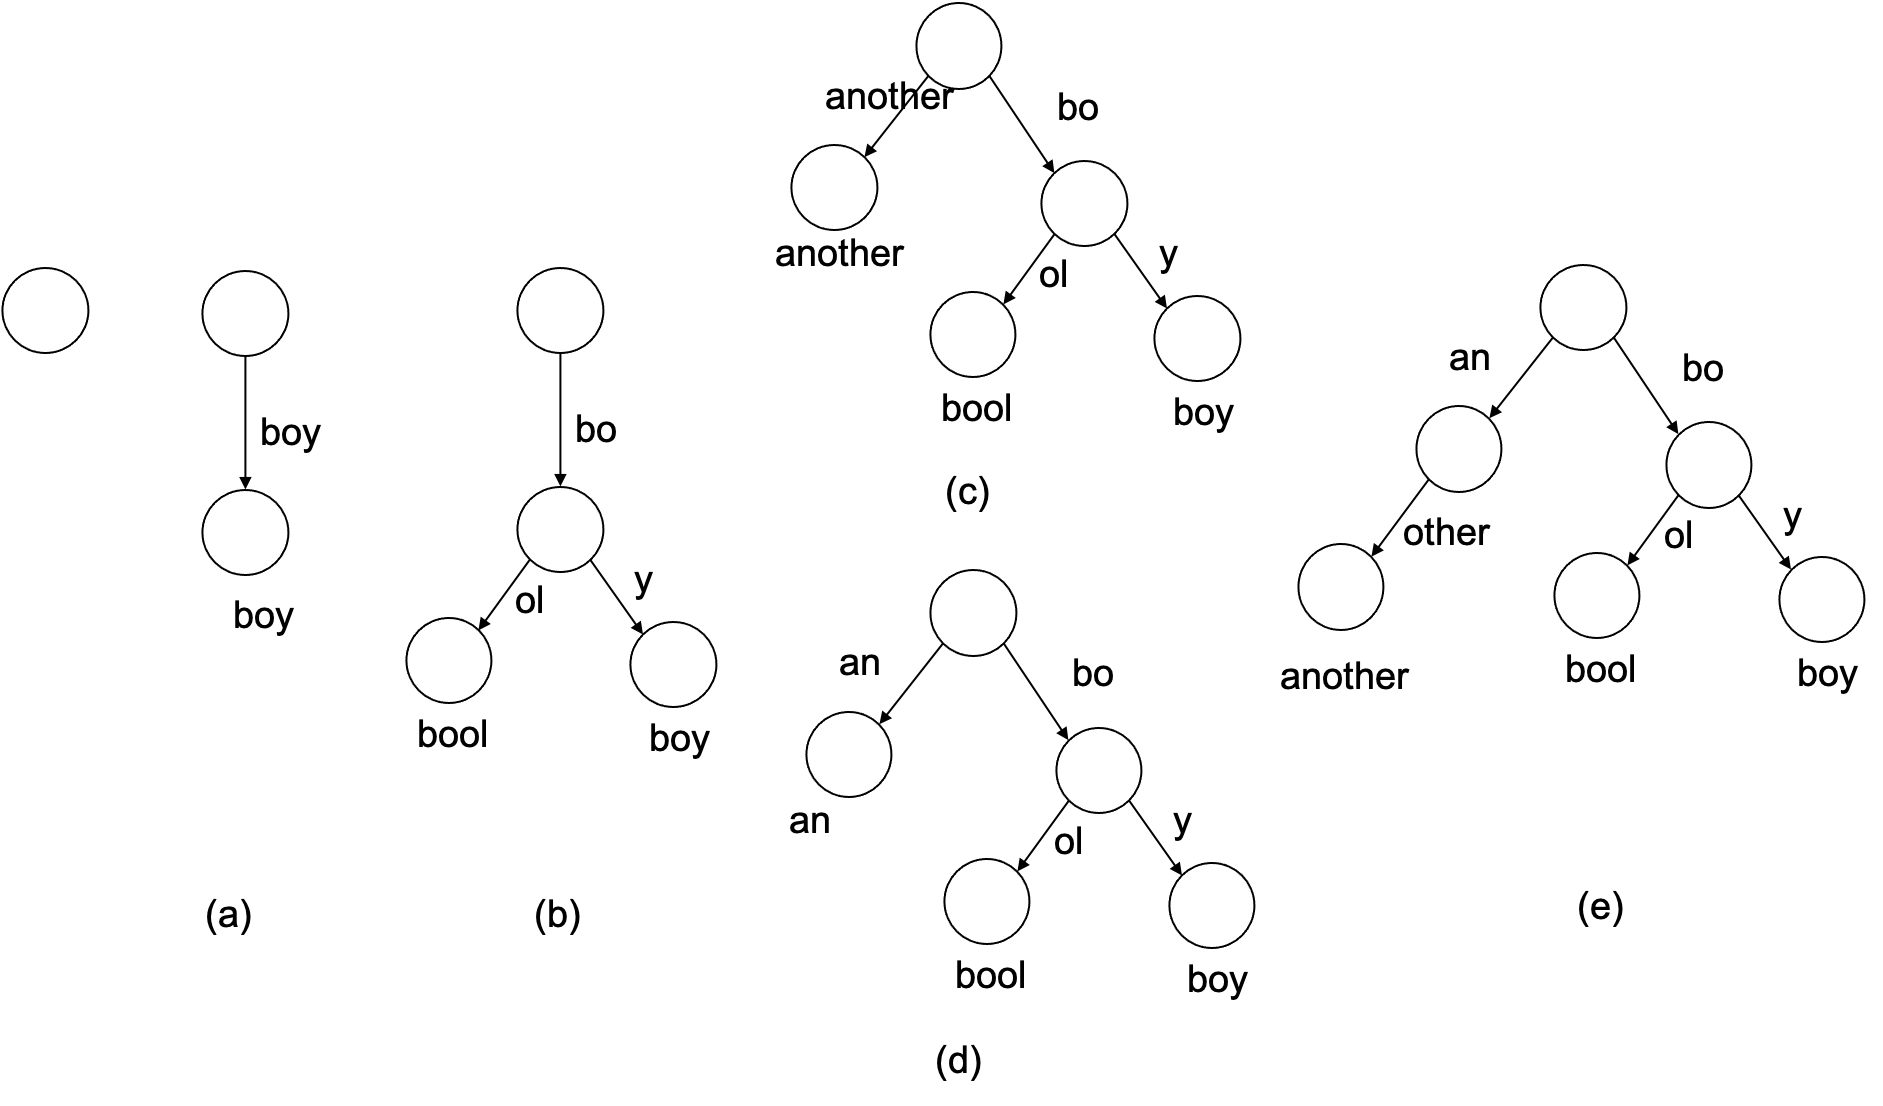
\includegraphics[scale=0.4]{img/prefix-tree-insert.png}
  \caption{(a) 向空树插入boy;(b) 插入bool,创建新分枝;(c) 向(b)插入another (d) 向(b)插入an (e) 向(c)插入an,结果与向(d)插入another相同}
  \label{fig:patricia-insert}
\end{figure}

下面的函数向前缀树$t = (v', ts)$中插入键$s$和值$v$:

\be
\begin{array}{rcl}
insert\ (v', ts)\ \nil\ v & = & (\textit{Just}\ v, ts) \\
insert\ (v', ts)\ s\ v & = & (v', ins\ ts) \\
\end{array}
\ee

如果键$s$为空,我们用$v$覆盖掉以前的值;否则调用$ins$检查子树和它们的前缀。

\be
\begin{array}{rcl}
ins\ \nil\ & = & [ s \mapsto (\textit{Just}\ v, \nil) ] \\
ins\ (s' \mapsto t) : ts' & = & \begin{cases}
  match\ s\ s': & (branch\ s\ v\ s'\ t) : ts' \\
  otherwise: & (s' \mapsto t) : ins\ ts' \\
  \end{cases}
\end{array}
\ee

如果节点不含任何子树,我们创建一个值为$v$的子树,并将$s$映射到其上;否则,对于每个子树映射$s' \mapsto t$,我们比较$s'$和$s$。如果它们有公共前缀(通过$match$函数检测),则利用$branch$函数分枝出子树。我们定义两个列表匹配如果它们有公共前缀:

\be
\begin{array}{rcl}
match\ \nil\ B & = & True \\
match\ A\ \nil & = & True \\
match\ (a:as)\ (b:bs) & = & a = b \\
\end{array}
\ee

我们定义函数$(C, A', B') = lcp\ A\ B$来提取列表$A$和$B$的最长公共前缀,其中$C \doubleplus A' = A$且$C \doubleplus B' = B$成立。如果$A$、$B$中的任何一个为空或者它们的第一个元素不同,则公共前缀$C = \nil$;否则,我们递归地从子列表中提取公共前缀,并将头部元素附加在前:

\be
\begin{array}{rcl}
lcp\ \nil\ B & = & (\nil, \nil, B) \\
lcp\ A\ \nil & = & (\nil, A, \nil) \\
lcp\ (a:as)\ (b:bs) & = & \begin{cases}
  a \neq b: & (\nil, a:as, b:bs) \\
  otherwise: & (a:cs, as', bs')\\
  \end{cases}
\end{array}
\ee

其中$(cs, as', bs') = lcp\ as\ bs$是递归提取的结果,函数$branch\ A\ v\ B\ t$接受两个键$A$、$B$,一个值$v$和树$t$,它提取出$A$、$B$的最长公共前缀$C$,将其映射到新分枝节点上,并设置好子树:

\be
\begin{array}{l}
branch\ A\ v\ B\ t = \\
\ lcp\ A\ B = \begin{cases}
   (C, \nil, B'): & (C, (\textit{Just}\ v, [B' \mapsto t])) \\
   (C, A', \nil): & (C, insert\ t\ A'\ v) \\
   (C, A', B'): & (C, (\textit{Nothing}, [A' \mapsto (\textit{Just}\ v, \nil), B' \mapsto t])) \\
\end{cases}
\end{array}
\ee

如果$A$是$B$的前缀,则将$A$映射到$v$所在的节点,列表的剩余部分被重新映射到分枝的唯一子树$t$;如果$B$是$A$的前缀,我们递归地将剩余列表和值插入到$t$中;否则,我们创建一个值为$v$的叶子节点,将其和$t$作为分枝的两棵子树。下面的例子程序实现了$insert$算法:

\begin{Haskell}
insert (PrefixTree _ ts) [] v = PrefixTree (Just v) ts
insert (PrefixTree v' ts) k v = PrefixTree v' (ins ts) where
    ins [] = [(k, leaf v)]
    ins ((k', t) : ts) | match k k' = (branch k v k' t) : ts
                       | otherwise  = (k', t) : ins ts

leaf v = PrefixTree (Just v) []

match [] _ = True
match _ [] = True
match (a:_) (b:_) = a == b

branch a v b t = case lcp a b of
  (c, [], b') -> (c, PrefixTree (Just v) [(b', t)])
  (c, a', []) -> (c, insert t a' v)
  (c, a', b') -> (c, PrefixTree Nothing [(a', leaf v), (b', t)])

lcp [] bs = ([], [], bs)
lcp as [] = ([], as, [])
lcp (a:as) (b:bs) | a /= b = ([], a:as, b:bs)
                  | otherwise = (a:cs, as', bs') where
                        (cs, as', bs') = lcp as bs
\end{Haskell}

我们也可以消除递归,用循环实现插入算法:

\begin{algorithmic}[1]
\Function{Insert}{$T, k, v$}
  \If{$T = $ NIL}
   \State $T \gets$ \Call{Empty-Node}{}
  \EndIf
  \State $p \gets T$
  \Loop
    \State $match \gets$ FALSE
    \For{each $s_i \mapsto T_i $ in \Call{Sub-Trees}{$p$}}
      \If{$k = s_i$}
        \State \Call{Value}{$T_i$} $\gets v$ \Comment{覆盖}
        \State \Return $T$
      \EndIf
      \State $c \gets$ \Call{LCP}{$k, s_i$}
      \State $k_1 \gets k - c$, $k_2 \gets s_i - c$
      \If{$c \neq $ NIL}
        \State $match \gets$ TRUE
        \If{$k_2 = $ NIL} \Comment{$s_i$是$k$的前缀}
          \State $p \gets T_i$, $k \gets k_1$
          \State break
        \Else \Comment{新分枝}
          \State \textproc{Add}(\Call{Sub-Trees}{$p$}, $c \mapsto$ \textproc{Branch}($k_1$, \Call{Leaf}{$v$}, $k_2$, $T_i$))
          \State \textproc{Delete}(\Call{Sub-Trees}{$p$}, $s_i \mapsto T_i$)
          \State \Return $T$
        \EndIf
      \EndIf
    \EndFor
    \If{not $match$} \Comment{新叶子}
      \State \textproc{Add}(\Call{Sub-Trees}{$p$}, $k \mapsto$ \Call{Leaf}{$v$})
      \State break
    \EndIf
  \EndLoop
  \State \Return $T$
\EndFunction
\end{algorithmic}

函数\textproc{LCP}提取出两个列表的公共前缀:

\begin{algorithmic}[1]
\Function{LCP}{$A, B$}
  \State $i \gets 1 $
  \While{$i \leq |A|$ and $i \leq |B|$ and $A[i] = B[i]$}
    \State $i \gets i + 1$
  \EndWhile
  \State \Return $A[1...i-1]$
\EndFunction
\end{algorithmic}

\textproc{Branch}($s_1, T_1, s_2, T_2$)中需要处理特殊情况。如果$s_1$为空,说明待插入的键是某个子树的前缀,我们将$T_2$设置为$T_1$的子树。否则,我们创建一个新的分枝节点,并将$T_1$、$T_2$设置为子树。

\begin{algorithmic}[1]
\Function{Branch}{$s_1, T_1, s_2, T_2$}
  \If{$s_1 = $ NIL}
    \State \textproc{Add}(\Call{Sub-Trees}{$T_1$}, $s_2 \mapsto T_2$)
    \State \Return $T_1$
  \EndIf
  \State $T \gets$ \Call{Empty-Node}{}
  \State \Call{Sub-Trees}{$T$} $\gets \{s_1 \mapsto T_1, s_2 \mapsto T_2\}$
  \State \Return $T$
\EndFunction
\end{algorithmic}

虽然前缀树提高了空间利用率,但其复杂度仍然是$O(mn)$,其中$n$是键的长度,$m$是列表元素集合的大小。

\subsection{查找}
\index{前缀树!查找}

查找键$k$时,我们从根节点开始,如果$k = \nil$为空,则返回根节点的值;否则我们检查子树的映射,找到映射$s_i \mapsto t_i$,使得$s_i$是$k$的前缀,然后再递归地在子树$t_i$中查找$k - s_i$。如果所有的$s_i$都不是$k$的前缀,则树中不存在要查找的键。

\be
\begin{array}{rcl}
lookup\ \nil\ (v, ts) & = & v \\
lookup\ k\ (v, ts) & = & find\ ((s, t) \mapsto s \sqsubseteq k)\ ts\ =  \\
  & & \begin{cases}
    \textit{Nothing} : & Nothing \\
    \textit{Just}\ (s, t): & lookup\ (k - s)\ t
  \end{cases}
\end{array}
\ee

其中$A \sqsubseteq B$表示$A$是$B$的前缀。函数$find$的定义见第一章,它在列表中查找满足指定条件的元素。下面的例子程序实现了查找算法。

\begin{Haskell}
lookup [] (PrefixTree v _) = v
lookup ks (PrefixTree v ts) =
  case find (\(s, t) -> s `isPrefixOf` ks) ts of
    Nothing -> Nothing
    Just (s, t) -> lookup (drop (length s) ks) t
\end{Haskell}

前缀检查所需的时间和列表的长度成比例,$lookup$算法的复杂度为$O(mn)$,其中$m$是列表元素集合的大小,$n$是列表的长度。我们略过了命令式实现,将其作为本节的练习。

\begin{Exercise}
\Question{消除$lookup$算法中的递归,用循环实现前缀树的查找。}
\end{Exercise}

\section{Trie和前缀树的应用}

我们可以用trie和前缀树来解决许多有趣的问题,包括实现简单的词典,自动输入补齐,以及数字键盘输入法。与商业实现不同,本节给出的例子都是示意性的。

\subsection{词典和自动补齐}
\index{自动补齐}

如图\ref{fig:e-dict}所示,当用户输入某些字符后,词典会搜索词库,列出候选单词。

\begin{figure}[htbp]
  \centering
  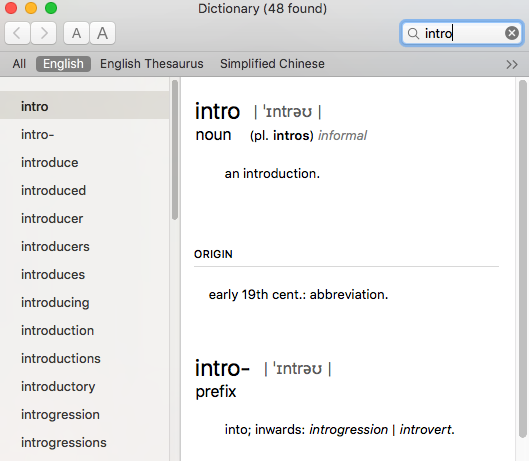
\includegraphics[scale=0.5]{img/edict-en.png}
  \caption{词典}
  \label{fig:e-dict}
\end{figure}

词典通常存有数十万单词,全部查找的开销很大。商业词典软件会使用多种工程方法以提高性能,包括缓存、索引等。图\ref{fig:word-completion}是一个带有自动补齐功能的输入框。当输入内容后,会列出一些可能的候选项。它们以用户输入的内容为前缀。

\begin{figure}[htbp]
  \centering
  
\includegraphics[scale=0.5]{img/adaptive-input.png}
  \caption{带有自动补齐的输入框}
  \label{fig:word-completion}
\end{figure}

这两个例子都展示了自动补齐的功能。我们可以用前缀树来实现它。简单起见,我们在例子中限定字符为英文,候选列表不超过$n$个条目。一个词典保存了多个键、值对,其中键是英文单词或词组,值是对应的意思和解释。当用户输入字符串$s$时,我们在前缀树实现的词典中查找所有以$s$开头的键。如果$s$为空,就扩展出所有子树直到达到$n$条结果;否则,我们根据匹配的子树递归查找。在支持惰性求值的环境中,我们可以扩展出全部候选项,然后按需取得前$n$个:$take\ n\ (startsWith\ s\ t)$,其中$t$是前缀树。

\be
\begin{array}{c}
\begin{array}{rcl}
startsWith\ \nil\ (\textit{Nothing}, ts) & = & enum\ ts \\
startsWith\ \nil\ (\textit{Just}\ x, ts) & = & (\nil, x) : enum\ ts \\
startsWith\ s\ (v, ts) & = & find\ ((k, t) \mapsto s \sqsubseteq k\ \text{or}\ k \sqsubseteq s)\ ts = \\
\end{array} \\
\quad \begin{cases}
  \textit{Nothing}: & \nil \\
  \textit{Just}\ (k, t): & [(k \doubleplus a, b) | (a, b) \in startsWith\ (s - k)\ t]
\end{cases}
\end{array}
\ee

给定一个列表$s$,函数$startsWith$在前缀树中搜索所有以$s$为前缀的结果。如果$s$为空,它枚举所有子树。如果根节点中的值$x$不为空,则将$(\nil, x)$附加到结果之前。函数$enum\ ts$定义如下:

\be
enum = \textit{concatMap}\ (k, t) \mapsto [(k \doubleplus a, b) | (a, b) \in startsWith\ \nil\ t]
\ee

其中$\textit{concatMap}$(也称为$flatMap$)是列表计算中的一个重要概念。效果上相当于先对每个元素进行映射,然后将结果连接起来。通常使用build-foldr融合律来实现,以消除计算中产生的中间结果列表(见《同构——编程中的数学》第5章)。如果$s$不为空,我们检查子树映射,对于每个映射$(k, t)$,如果$s$或$k$是另外一个的前缀,我们就递归地扩展子树$t$,并将$k$附加到每个结果的键之前;否则,如果$s$不和任何子树的映射匹配,则不存在以$s$为前缀的结果。下面的例子程序实现了这一算法:

\begin{Haskell}
startsWith [] (PrefixTree Nothing ts) = enum ts
startsWith [] (PrefixTree (Just v) ts) = ([], v) : enum ts
startsWith k (PrefixTree _ ts) =
  case find (\(s, t) -> s `isPrefixOf` k || k `isPrefixOf` s) ts of
    Nothing -> []
    Just (s, t) -> [(s ++ a, b) |
                         (a, b) <- startsWith (drop (length s) k) t]

enum = concatMap (\(k, t) -> [(k ++ a, b) | (a, b) <- startsWith [] t])
\end{Haskell}

我们也可以用命令式的方式实现\textproc{Starts-With}($T, k, n$)。从根节点开始,我们循环检查每个子树映射$k_i \mapsto T_i$。如果$k$是某个子树$T_i$的前缀,我们就将这棵子树扩展到最多$n$条结果;如果$k_i$是$k$的前缀,我们就去掉前缀部分,用新键$k - k_i$在$T_i$中递归查找。

\begin{algorithmic}[1]
\Function{Starts-With}{$T, k, n$}
  \If{$T = $ NIL}
     \State \Return NIL
  \EndIf
  \State $s \gets$ NIL
  \Repeat
    \State $match \gets$ FALSE
    \For{$k_i \mapsto T_i$ in \Call{Sub-Trees}{$T$}}
      \If{$k$ is prefix of $k_i$}
        \State \Return \Call{Expand}{$s \doubleplus k_i, T_i, n$}
      \EndIf
      \If{$k_i$ is prefix of $k$}
        \State $match \gets$ TRUE
        \State $k \gets k - k_i$  \Comment{去掉前缀}
        \State $T \gets T_i$
        \State $s \gets s \doubleplus k_i$
        \State break
      \EndIf
    \EndFor
  \Until{not $match$}
  \State \Return NIL
\EndFunction
\end{algorithmic}

其中函数\textproc{Expand}($s, T, n$)从$T$中扩展出$n$个结果,并将$s$附加在每个键的前面。我们可以用广度优先搜索方法实现它(见14.3节):

\begin{algorithmic}[1]
\Function{Expand}{$s, T, n$}
  \State $R \gets $ NIL
  \State $Q \gets [(s, T)]$
  \While{$|R| < n$ and $Q \neq$ NIL}
    \State $(k, T) \gets$ \Call{Pop}{$Q$}
    \State $v \gets$ \Call{Value}{$T$}
    \If{$v \neq$ NIL}
      \State \Call{Insert}{$R, (k, v)$}
    \EndIf
    \For{$k_i \mapsto T_i$ in \Call{Sub-Trees}{$T$}}
      \State \Call{Push}{$Q, (k \doubleplus k_i, T_i)$}
    \EndFor
  \EndWhile
\EndFunction
\end{algorithmic}


\subsection{数字键盘输入法}
\index{T9}

2010年前,大多数手机上都提供一个如图\ref{fig:itut-keypad}所示的数字键盘,称为ITU-T键盘。它将每个数字映射到3到4个英文字母上。如果要输入英文单词home,我们可以按照下面的顺序按键:

\begin{figure}[htbp]
  \centering
  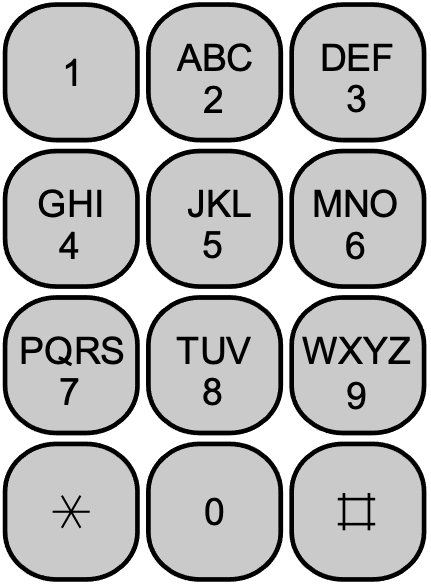
\includegraphics[scale=0.4]{img/itu-t.png}
  \caption{手机ITU-T键盘}
  \label{fig:itut-keypad}
\end{figure}

\begin{enumerate}
\item 按两次4键输入字符h;
\item 按三次6键输入字符o;
\item 按一次6键输入字符m;
\item 按两次3键输入字符e;
\end{enumerate}

另外一种更快速的方法使用下面的按键顺序:

\begin{enumerate}
\item 依次按下4、6、6、3,候选单词home出现;
\item 按下‘*’号键以变换到下一个候选单词good;
\item 按下‘*’号键再次变换到下一个候选单词gone;
\item ……
\end{enumerate}

后者称为预测式输入,简称为T9\cite{wiki-t9}、\cite {wiki-predictive-text}。商业实现通常在内存和文件系统中使用多级缓存和索引。作为示例,我们可以将单词存储在一个前缀树中来实现这种输入法。首先我们需要定义数字键盘映射:

\be
\begin{array}{ll}
M_{T9} = \{ & 2 \mapsto \texttt{"abc"}, 3 \mapsto \texttt{"def"}, 4 \mapsto \texttt{"ghi"}, \\
           & 5 \mapsto \texttt{"jkl"}, 6 \mapsto \texttt{"mno"}, 7 \mapsto \texttt{"pqrs"}, \\
           & 8 \mapsto \texttt{"tuv"}, 9 \mapsto \texttt{"wxyz"} \quad \}
\end{array}
\ee

$M_{T9}[i]$就给出数字$i$对应的若干字符。我们也可以定义从字符到数字的逆映射。

\be
M^{-1}_{T9} = \textit{concatMap}\ ((d, s) \mapsto [(c, d) | c \in s])\ M_{T9}
\ee

通过查找$M^{-1}_{T9}$,我们可以将字符串转换成一组按键序列。

\be
digits(s) = \{ M^{-1}_{T9}[c]| c \in s \}
\ee

对于任何不属于[\texttt{a..z}]中的字符,我们将其映射到特殊字符\texttt{'\#'}上。下面的例子程序定义了上述映射:

\begin{Haskell}
mapT9 = Map.fromList [('2', "abc"), ('3', "def"), ('4', "ghi"),
                      ('5', "jkl"), ('6', "mno"), ('7', "pqrs"),
                      ('8', "tuv"), ('9', "wxyz")]

rmapT9 = Map.fromList $ concatMap (\(d, s) -> [(c, d) | c <- s]) $
           Map.toList mapT9

digits = map (\c -> Map.findWithDefault '#' c rmapT9)
\end{Haskell}

令$(v, ts)$是从所有候选单词构建出的前缀树。我们可以修改自动补齐算法来处理数字序列$ds$。我们把每个子树映射$(s \mapsto t) \in ts$中的前缀$s$转换为$digits(s)$,检查它是否和$ds$匹配(其中一个为另一个的前缀)。可能存在多个子树匹配$ds$的情况:

\[
\textit{pfx} = [(s, t) | (s \mapsto t) \in ts, digits(s) \sqsubseteq ds\ \textit{or}\ ds\ \sqsubseteq digits(s)]
\]

\be
\begin{array}{rcl}
find_{T9}\ t\ \nil & = & [ \nil ] \\
find_{T9}\ (v, ts)\ ds & = & \textit{concatMap}\ find\ \textit{pfx} \\
\end{array}
\ee

对\textit{pfx}中的每个映射$(s, t)$,函数$find$递归地在$t$中查找剩余数字$ds'$,其中$ds' = drop\ |s|\ ds$,然后将$s$附加到每个候选项前面。为了防止长度超出数字个数,我们截取前$n = |ds|$个字符:

\be
find\ (s, t) = [ take\ n\ (s \doubleplus s_i) | s_i \in find_{T9}\ t\ ds']
\ee

下面的例子程序实现了预测输入法:

\begin{Haskell}
findT9 _ [] = [[]]
findT9 (PrefixTree _ ts) k = concatMap find pfx where
  find (s, t) = map (take (length k) . (s++)) $ findT9 t (drop (length s) k)
  pfx = [(s, t) | (s, t) <- ts, let ds = digits s in
              ds `isPrefixOf` k || k `isPrefixOf` ds]
\end{Haskell} %$

用命令式方法实现广度优先搜索时,可以用一个队列$Q$,队列中的元素为三元组$(\textit{prefix}, D, t)$。每个三元组包含已搜索过的前缀\textit{prefix},尚未搜索的数字$D$,和待搜索的子树$t$。队列初始的时候,三元组包含空前缀,全部数字,以及前缀树的根节点。我们不断从队列中取出三元组,检查子树的映射。对于每个映射$(s \mapsto T')$,我们将$s$转换成$digits(s)$。如果$D$是它的前缀,就找到了一个候选词。我们将$s$附加到\textit{prefix}的前面,并记录下这一结果。如果$digits(s)$是$D$的前缀,我们需要递归在子树$T'$中搜索,我们新建一个三元组$(\textit{prefix} \doubleplus s, D', T')$,其中$D'$是剩余的数字。然后将这一新三元组放回队列。

\begin{algorithmic}[1]
\Function{Look-Up-T9}{$T, D$}
  \State $R \gets $ NIL
  \If{$T =$ NIL or $D =$ NIL}
    \State \Return $R$
  \EndIf
  \State $n \gets |D|$
  \State $Q \gets \{(\text{NIL}, D, T)\}$
  \While{$Q \neq $ NIL}
    \State $(\textit{prefix}, D, T) \gets$ \Call{Pop}{$Q$}
    \For{$(s \mapsto T') \in $ \Call{Sub-Trees}{$T$}}
      \State $D' \gets$ \Call{Digits}{$s$}
      \If{$D' \sqsubset D$} \Comment{$D'$是$D$的前缀}
        \State \Call{Append}{$R, (\textit{prefix} \doubleplus s)[1..n]$} \Comment{限制长度为$n$}
      \ElsIf{$D \sqsubset D'$}
        \State \Call{Push}{$Q, (\textit{prefix} \doubleplus s, D - D', T')$}
      \EndIf
    \EndFor
  \EndWhile
  \State \Return $R$
\EndFunction
\end{algorithmic}

\begin{Exercise}
\Question{使用trie实现自动补齐和预测式输入。}
\Question{对于返回多个候选结果的前缀树查找算法,如何保证输出的结果按照字典顺序排序?这会对性能产生怎样的影响?}
\Question{在没有惰性求值的环境中,如何按需返回最多$n$条结果?}
\end{Exercise}

\section{小结}
我们从整数trie和整数前缀树开始,通过整数的二进制表示,我们复用二叉树实现了基于整数的映射(map)数据结构。接下来我们将键的类型从整数扩展到有限集元素的列表。其中一个特例就是字符串,trie和前缀树可以用来进行文字处理。我们给出了两个应用的例子:自动补齐和预测式输入。基数树的另外一个应用是后缀树,它和trie与前缀树有着密切的关系,是文字和DNA处理的有力工具。

\section{附录:例子程序}

复用二叉树定义整数trie:

\begin{lstlisting}[language = Bourbaki]
data IntTrie<T> {
    IntTrie<T> left = null
    IntTrie<T> right = null
    Optional<T> value = Optional.None
}
\end{lstlisting}

下面的$insert$例子程序用位运算实现了奇偶测试和向右移位:

\begin{lstlisting}[language = Bourbaki]
IntTrie<T> insert(IntTrie<T> t, Int key,
                  Optional<T> value = Optional.None) {
    if t == null then t = IntTrie<T>()
    p = t
    while key != 0 {
        if key & 1 == 0 {
            p = if p.left == null then IntTrie<T>() else p.left
        } else {
            p = if p.right == null then IntTrie<T>() else p.right
        }
        key = key >> 1
    }
    p.value = Optional.of(value)
    return t
}
\end{lstlisting}

%% Integer trie lookup:

%% \begin{lstlisting}[language = Bourbaki]
%% Optional<T> lookup(IntTrie<T> t, Int key) {
%%     while t != null and k != 0 {
%%         t = if key & 1 == 0 then t.left else t.right
%%         key = key >> 1
%%     }
%%     return if t == null then Optional.None else t.value
%% }
%% \end{lstlisting}

整数前缀树的定义:

\begin{lstlisting}[language = Bourbaki]
data IntTree<T> {
    Int key
    T value
    Int prefix
    Int mask = 1
    IntTree<T> left = null
    IntTree<T> right = null

    IntTree(Int k, T v) {
        key = k, value = v, prefix = k
    }

    bool isLeaf = (left == null and right == null)

    Self replace(IntTree<T> x, IntTree<T> y) {
        if left == x then left = y else right = y
    }

    bool match(Int k) = maskbit(k, mask) == prefix
}

Int maskbit(Int x, Int mask) = x & (~(mask - 1))
\end{lstlisting}

向整数前缀树插入键、值:

\begin{lstlisting}[language = Bourbaki]
IntTree<T> insert(IntTree<T> t, Int key, T value) {
    if t == null then return IntTree(key, value)
    node = t
    Node<T> parent = null
    while (not node.isLeaf()) and node.match(key) {
        parent = node
        node = if zero(key, node.mask) then node.left else node.right
    }
    if node.isleaf() and key == node.key {
        node.value = value
    } else {
        p = branch(node, IntTree(key, value))
        if parent == null then return p
        parent.replace(node, p)
    }
    return t
}

IntTree<T> branch(IntTree<T> t1, IntTree<T> t2) {
    var t = IntTree<T>()
    (t.prefix, t.mask) = lcp(t1.prefix, t2.prefix)
    (t.left, t.right) = if zero(t1.prefix, t.mask) then (t1, t2)
                        else (t2, t1)
    return t
}

bool zero(int x, int mask) = (x & (mask >> 1) == 0)

Int lcp(Int p1, Int p2) {
    Int diff = p1 ^ p2
    Int mask = 1
    while diff != 0 {
        diff = diff >> 1
        mask = mask << 1
    }
    return (maskbit(p1, mask), mask)
}
\end{lstlisting}

%% \begin{lstlisting}[language = Bourbaki]
%% Optional<Node<T>> lookup(Node<T> t, Int key) {
%%     while t != null and (not t.isLeaf()) and t.match(key) {
%%         t = if zero(key, t.mask) then t.left else t.right
%%     }
%%     return if t != null and t.isLeaf() and t.key == key
%%            then Optional.of(t.value) else Optional.None
%% }
%% \end{lstlisting}

trie的定义和插入:

\begin{lstlisting}[language = Bourbaki]
data Trie<K, V> {
  Optional<V> value = Optional.None
  Map<K, Trie<K, V>> subTrees = Map.empty()
}

Trie<K, V> insert(Trie<K, V> t, [K] key, V value) {
    if t == null then t = Trie<K, V>()
    var p = t
    for c in key {
        if p.subTrees[c] == null then p.subTrees[c] = Trie<K, V>()
        p = p.subTrees[c]
    }
    p.value = Optional.of(value)
    return t
}
\end{lstlisting}

前缀树的定义和插入:

\begin{lstlisting}[language = Bourbaki]
data PrefixTree<K, V> {
    Optional<V> value = Optional.None
    Map<[K], PrefixTree<K, V>> subTrees = Map.empty()

    Self PrefixTree(V v) {
        value = Optional.of(v)
    }
}

PrefixTree<K, V> insert(PrefixTree<K, V> t, [K] key, V value) {
    if t == null then t = PrefixTree()
    var node = t
    loop {
        bool match = false
        for var (k, tr) in node.subtrees {
            if key == k {
                tr.value = value
                return t
            }
            prefix, k1, k2 = lcp(key, k)
            if prefix != [] {
                match = true
                if k2 == [] {
                    node = tr
                    key = k1
                    break
                } else {
                    node.subtrees[prefix] = branch(k1, PrefixTree(value),
                                                   k2, tr)
                    node.subtrees.delete(k)
                    return t
                }
            }
        }
        if !match {
            node.subtrees[key] = PrefixTree(value)
            break
        }
    }
    return t
}
\end{lstlisting}

提取最长公共前缀\texttt{lcp}和分枝\texttt{branch}:

\begin{lstlisting}[language = Bourbaki]
([K], [K], [K]) lcp([K] s1, [K] s2) {
    j = 0
    while j < length(s1) and j < length(s2) and s1[j] == s2[j] {
        j = j + 1
    }
    return (s1[0..j-1], s1[j..], s2[j..])
}

PrefixTree<K, V> branch([K] key1, PrefixTree<K, V> tree1,
                        [K] key2, PrefixTree<K, V> tree2) {
    if key1 == []:
        tree1.subtrees[key2] = tree2
        return tree1
    t = PrefixTree()
    t.subtrees[key1] = tree1
    t.subtrees[key2] = tree2
    return t
}
\end{lstlisting}

枚举共同前缀的所有候选项:

\begin{lstlisting}[language = Bourbaki]
[([K], V)] startsWith(PrefixTree<K, V> t, [K] key, Int n) {
    if t == null then return []
    [T] s = []
    repeat {
        bool match = false
        for var (k, tr) in t.subtrees {
            if key.isPrefixOf(k) {
                return expand(s ++ k, tr, n)
            } else if k.isPrefixOf(key) {
                match = true
                key = key[length(k)..]
                t = tr
                s = s ++ k
                break
            }
        }
    } until not match
    return []
}

[([K], V)] expand([K] s, PrefixTree<K, V> t, Int n) {
    [([K], V)] r = []
    var q = Queue([(s, t)])
    while length(r) < n and !q.isEmpty() {
        var (s, t) = q.pop()
        v = t.value
        if v.isPresent() then r.append((s, v.get()))
        for k, tr in t.subtrees {
            q.push((s ++ k, tr))
        }
    }
    return r
}
\end{lstlisting}

预测式输入:
\begin{lstlisting}[language = Bourbaki]
var T9MAP={'2':"abc", '3':"def", '4':"ghi", '5':"jkl", \
       '6':"mno", '7':"pqrs", '8':"tuv", '9':"wxyz"}

var T9RMAP = { c : d for var (d, cs) in T9MAP for var c in cs }

string digits(string w) = ''.join([T9RMAP[c] for c in w])

[string] lookupT9(PrefixTree<char, V> t, string key) {
    if t == null or key == "" then return []
    res = []
    n = length(key)
    q = Queue(("", key, t))
    while not q.isEmpty() {
        (prefix, key, t) = q.pop()
        for var (k, tr) in t.subtrees {
            ds = digits(k)
            if key.isPrefixOf(ds) {
                res.append((prefix ++ k)[:n])
            } else if ds.isPrefixOf(key) {
                q.append((prefix ++ k, key[length(k)..], tr))
            }
        }
    }
    return res
}
\end{lstlisting}

\ifx\wholebook\relax\else
\begin{thebibliography}{99}

\bibitem{CLRS}
Thomas H. Cormen, Charles E. Leiserson, Ronald L. Rivest and Clifford Stein.
``Introduction to Algorithms, Second Edition''. Problem 12-1. ISBN:0262032937. The MIT Press. 2001(《算法导论》)

\bibitem{okasaki-int-map}
Chris Okasaki and Andrew Gill. ``Fast Mergeable Integer Maps''. Workshop on ML, September 1998, pages 77-86.  \url{http://www.cse.ogi.edu/~andy/pub/finite.htm}

\bibitem{patricia-morrison}
D.R. Morrison, ``PATRICIA -- Practical Algorithm To Retrieve  Information Coded In Alphanumeric", Journal of the ACM, 15(4), October 1968, pages 514-534.

\bibitem{wiki-suffix-tree}
Suffix Tree, Wikipedia. \url{https://en.wikipedia.org/wiki/Suffix_tree}

\bibitem{wiki-trie}
Trie, Wikipedia. \url{https://en.wikipedia.org/wiki/Trie}

\bibitem{wiki-t9}
T9 (predictive text), Wikipedia. \url{https://en.wikipedia.org/wiki/T9_(predictive_text)}

\bibitem{wiki-predictive-text}
Predictive text,
Wikipedia. \url{https://en.wikipedia.org/wiki/Predictive_text}

\end{thebibliography}

\end{document}
\fi
